\subsubsection*{Cost Category 22.01.01 First Wall and Blanket} 

The first wall in a fusion heat island serves as a direct interface with the plasma, tasked with withstanding extreme heat and particle flux while also resisting radiation damage and managing tritium retention. The blanket surrounding the first wall plays a dual role in absorbing neutrons to generate heat and breed tritium for fuel, in addition to providing crucial radiation shielding for the reactor's structural integrity and safety.  This Cost Category therefore consists of the following subcategories:

%https://docs.google.com/spreadsheets/d/1SlP_hoDTWUznvav6WUs5kozBXcQWKO2okvEGQukS6Mw/edit#gid=476735038

\begin{itemize}
    \item Cost Category 21.01.01 First wall: the interior surface of the fusion chamber that directly faces the plasma and is subject to extreme conditions. It endures intense heat and particle flux, necessitating the use of materials like refractory metals or specialized alloys that can withstand high temperatures and minimize erosion from particle bombardment. The first wall must also resist radiation damage, particularly in deuterium-tritium fusion reactors, where neutron radiation can cause materials to become brittle and lose structural integrity. An important consideration is the management of tritium retention and release, as wall materials should prevent buildup while allowing efficient extraction and reuse. Additionally, the first wall faces significant thermal stress due to the cyclic nature of fusion reactions, requiring a design that can accommodate stresses without cracking or deforming. Finally, it must be compatible with the cooling system, which could involve water, liquid metal, or other coolants, to ensure effective heat removal. The design and performance of the first wall are critical for the reactor's efficiency, safety, and longevity, which presents a complex engineering challenge that balances heat resistance, structural integrity, and minimal plasma interaction.
    \item Cost Category 21.01.02 Blanket: a crucial component that surrounds the plasma, serving multiple roles. It absorbs neutrons generated during fusion reactions, converting their kinetic energy into heat, and acts as a breeding ground for tritium, an essential fuel in deuterium-tritium fusion reactions, through interactions with materials like lithium. The blanket also provides critical radiation shielding, protecting reactor components and personnel from intense neutron radiation. Additionally, it plays a role in thermal management, as the heat generated within the blanket is often harnessed to produce steam for driving turbines and generating electricity. This makes the design and material choice for the blanket vital for reactor efficiency and safety, which requires advanced materials and engineering to withstand extreme temperatures and radiation levels.
\end{itemize}

The blanket under consideration has a liquid lithium first wall with a primary coolant consisting of Lead Lithium (PbLi) and water as the secondary coolant, with Pb as part of PbLi as the neutron multiplier, and a structure primarily consisting of Ferritic Martensitic Steel (FMS). The radial build dimensions are shown in Table \ref{tab:volumes}, which allow us to determine the volumes of components for costing.  The radial build is shown in \ref{fig:radial}.  \\


\begin{table}[h!]
    \centering
    \begin{tabular}{l c  c c c}
    \hline
        &	Thickness	&	Inner Radius	&	Outer radius	&	Volume		\\
        \hline
Plasma	&	1.1	&	3.0	&	4.1	&	215.0	m$^{3}$	\\
Vacuum	&	0.1	&	4.1	&	4.2	&	40.9	m$^{3}$	\\
First Wall	&	0.2	&	4.2	&	4.4	&	92.4	m$^{3}$	\\
Blanket	&	0.8	&	4.4	&	5.2	&	512.0	m$^{3}$	\\
Reflector	&	0.2	&	5.2	&	5.4	&	163.0	m$^{3}$	\\
HT Shield	&	0.2	&	5.4	&	5.6	&	178.0	m$^{3}$	\\
Structure	&	0.2	&	5.6	&	5.8	&	192.0	m$^{3}$	\\
Gap	&	0.5	&	5.8	&	6.3	&	542.0	m$^{3}$	\\
Vessel	&	0.2	&	6.3	&	6.5	&	242.0	m$^{3}$	\\
LT Shield	&	0.2	&	5.4	&	5.6	&	178.0	m$^{3}$	\\
Coils	&	0.3	&	6.5	&	6.85	&	389.0	m$^{3}$	\\
Structure	&	0.05	&	6.8	&	6.85	&	439.0	m$^{3}$	\\
Gap	&	0.3	&	6.5	&	6.8	&	389.0	m$^{3}$	\\
Bioshield	&	0.5	&	6.85	&	7.35	&	1120.0	m$^{3}$	\\

        \hline
    \end{tabular}
    \caption{Volumes of components in the radial build.}
    \label{tab:volumes}
\end{table}

\begin{figure}
    \centering
    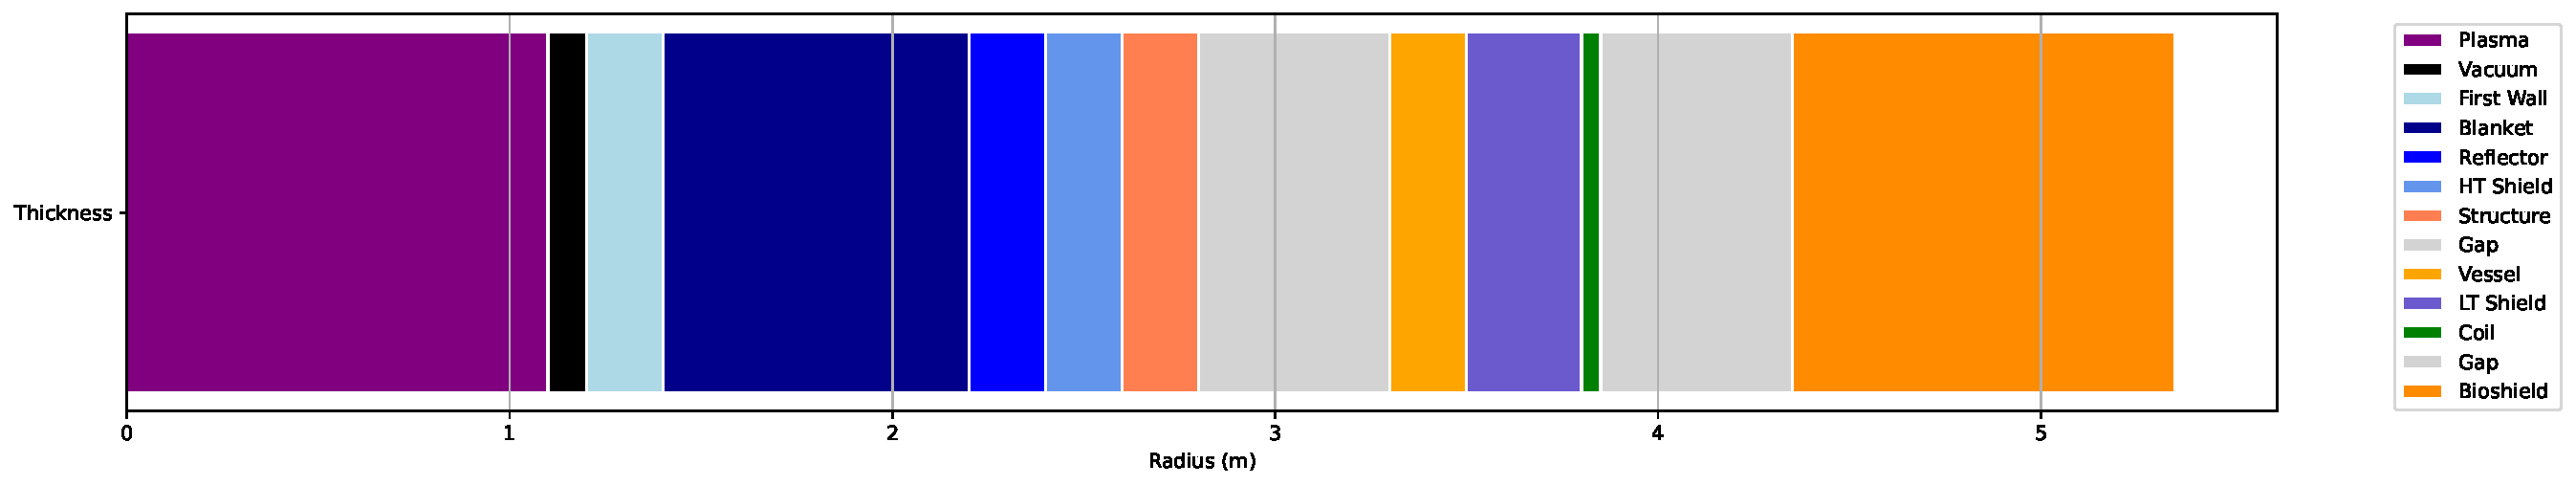
\includegraphics[width=0.9\linewidth]{Figures/radial_build.pdf}
    \caption{Radial build according to Table \ref{tab:volumes}.}
    \label{fig:radial}
\end{figure}



The costs of the first wall and blanket are determined by the volume of the material and multiplied by a manufacturing factor per Table \ref{tab:materials}.   Cost of the first wall is \$ 5.2 M.  Cost of the blanket is \$ 29.0 M. The total is therefore \$ 34.0 M.

